% Basic setup 

A flow configuration that combines the complexities of high density-ratios with the interaction between capillary, viscous and inertial stresses is that of a water droplet falling in air under the influence of gravitational acceleration. The problem is characterized by a combination of Reynolds, Weber and Bond numbres, the definitions of which are as follows : 

\begin{align}
We=\frac{\rho_{\rm air} U^2 d}{\sigma} \quad,\quad Re= \frac{\rho_{\rm air} U d}{\mu_{\rm air}} \quad,\quad Bo=\frac{\left(\rho_{\rm wat}-\rho_{\rm air}\right) g d^2 }{\sigma}
\end{align}

\vspace*{0.2cm}

In our particular numerical setup, $We \simeq 3.2 $, $Re \simeq 1455 $ and $Bo \simeq 1.0 $, thus corresponding to that of a $3mm$ diameter raindrop (a relatively large one) falling in air at an approximate terminal velocity of  $8 m/s$ (interpolated from empirical data, refer to  \cite{gunn1949terminal}). The parameters in the problem setup is given in Table \ref{raindropprop}, and the schematic diagram given by Fig. \ref{setup}. The droplet is initially placed at the center of a cubic domain (3D), whose side is 4 times the diameter of the drop. 

\vspace*{0.2cm}

% -----
\begin{table}[h!]
\begin{center}
\begin{tabular}{ccccccc}
\hline\hline
$\rho_{\rm air}$ & $\rho_{\rm water}$ & $\mu_{\rm air}$ 
& $\mu_{\rm water}$ & $\sigma$ & $d$ & $g$\\
$\left(kg/m^3\right)$ & $\left(kg/m^3\right)$ & $\left(Pa \, s\right)$ 
& $\left(Pa \,s \right)$ & $\left(N/m\right)$ & $(m)$ & $(m /s^{2})$ \\
\hline
1.2 & $0.9982\, 10^3$ & $1.98\,10^{-5}$ & 
$8.9 \, 10^{-4}$ & $0.0728$ & $3\, 10^{-3}$ & $9.81$\\
\hline\hline
\end{tabular}
\caption{Parameter values used in the simulation of a falling water droplet in air. \label{raindropprop}}
\end{center}
\end{table}
% -----

\vspace*{0.2cm}

In order to properly reproduce and analyse the dynamics of a relatively large drop (high Reynolds flow) such as in our case, the numerical method has to accurately resolve the thin, complicated boundary layers, the interaction of such layers with the capillary deformations and finally the non-linear feedback of the complex 3D vortical structures in the droplet wake to the surrounding pressure field. Therefore, we explicitly state that the aim of this particular test case is not to develop a high fidelity model of a raindrop, but rather carry out a stringent evaluation of the robustness of our numerical method compared to methods which are not momentum consistent. For such a low Weber number the capillary forces dominate and the droplet should remain approximately spherical, and should definitely not undergoe any subsequent atomization. 


% -----
\begin{figure}[h!]
\begin{center}
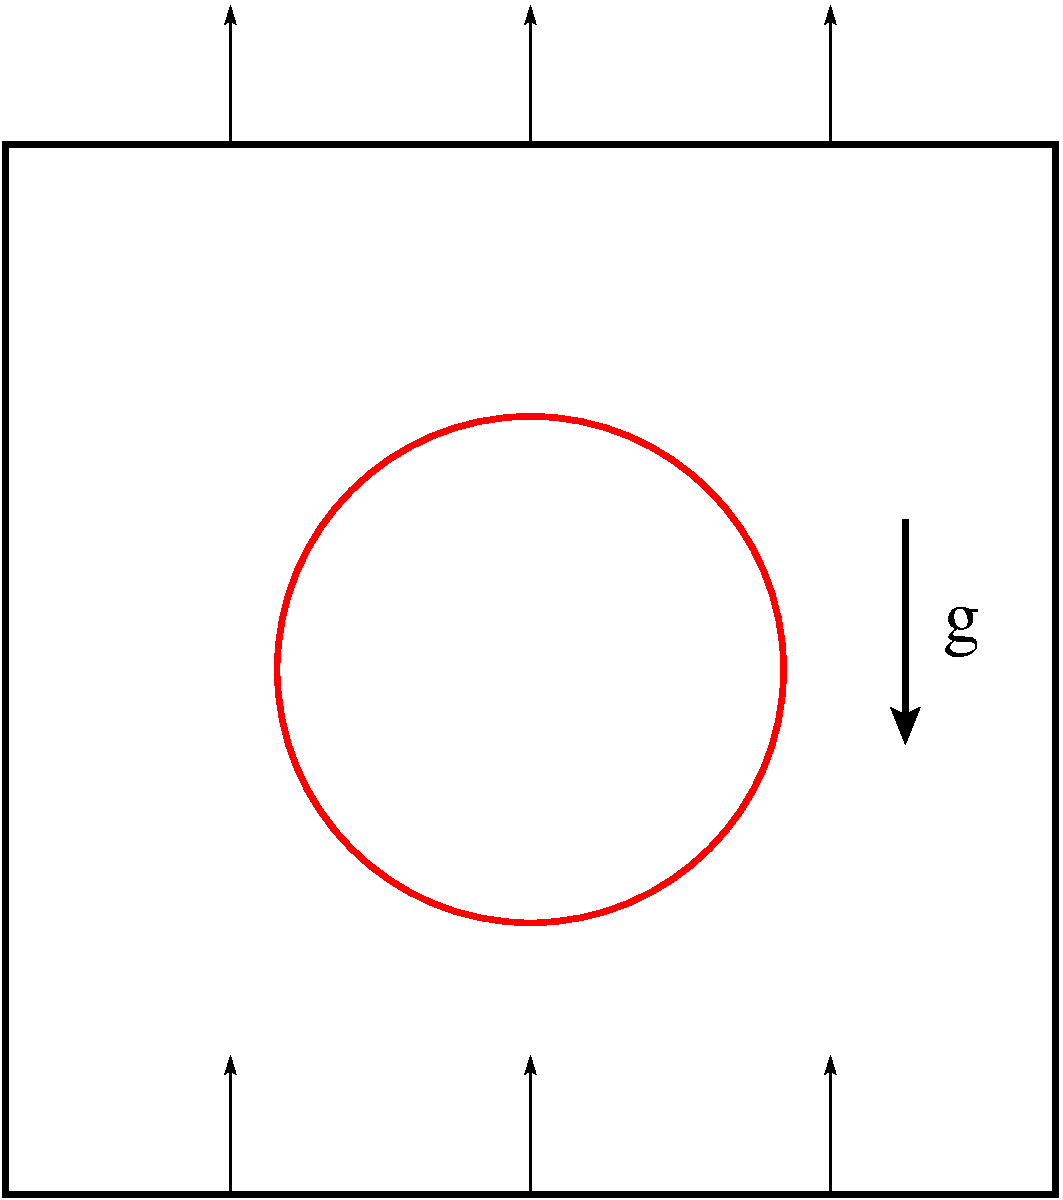
\includegraphics[width=0.35\textwidth]{Figures/setup.pdf}
\end{center}
\caption{Problem setup for falling rain drop test case. Boundary conditions 
at the top and bottom are a uniform inflow and outflow velocity $U_0(t)$. 
Boundary conditions on the side are free slip (no shear stress).}
\label{setup}
\end{figure}
% -----


% -----
\begin{figure}
\begin{center}
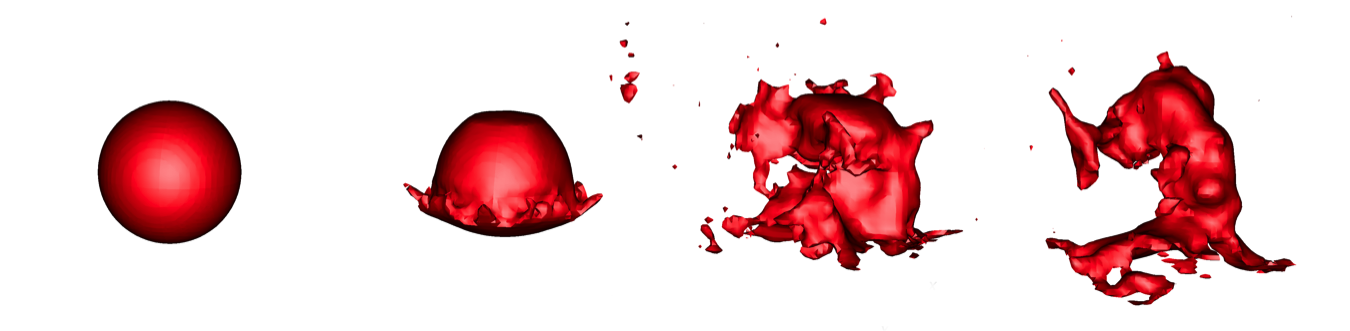
\includegraphics[width=0.75\textwidth]{Figures/cata.png}
\end{center}
\caption{Rain drop test case: catastrophic breakup with non-conserving 
formulation, $D/h=30$.}
\label{cata}
\end{figure}
% -----

Numerical simulations of this test case at moderate resolution ($D/h=16$ to 64 grid points per diameter were tested) without the consistent momentum-conserving scheme described in this paper, results in the catastrophic deformations of the droplet as shown in Fig. \ref{cata}, which we like to describe as 'fictitious' atomization as a result of rapidly growing numerical instabilities. This effect was previously uncovered by \cite{Xiao:2014vs} in a similar case involcing the sudden interaction of a droplet at rest with a uniform gas flow. The Weber number in that case was also around 3, therefore rendering the droplet nearly spherical but ref. \cite{Xiao:2014vs} reports a similar catastrophic deformation and gives the following explanation. To start with, we neglect gravity and viscous effects at this relatively large Reynolds number. Also, we are interested in steady-state flow. On the axis and near the hyperbolic stagnation point at the front of the droplet one has $u_2=0$ for the transverse (radial) velocity and for the axial momentum balance

\be
u_1 \partial_1 u_1 = - \frac 1 \rho \partial_1 p.
\nd

Because of the low viscosity and large density ratio, it is not possible for the air flow to immediately entrain the water, so the fluid velocity is significantly smaller in the water. In the air the acceleration near the stagnation point is $U^2/D$ and the pressure gradient is

\be
\partial_1 p \sim \rho_{a} U^2/D.
\nd
The pressure gradient in the water is much smaller, however if in a mixed cell the water density multiplies the air acceleration $U^2/D$, so that
\be
\partial_1 p \sim \rho_{w} U^2/D,
\nd

then a large pressure gradient results in the mixed cell or cells. This large pressure gradient results in a large pressure inside the droplet near the front stagnation point, as shown in Figure \ref{FengXiao}. This large pressure is balanced by surface tension only for a sufficiently large curvature near the droplet front. This explains the presence of a ``dimple'' often observed in low resolution simulations of the falling drop. 

% -----
\begin{figure}
\begin{center}
\begin{tabular}{cc}
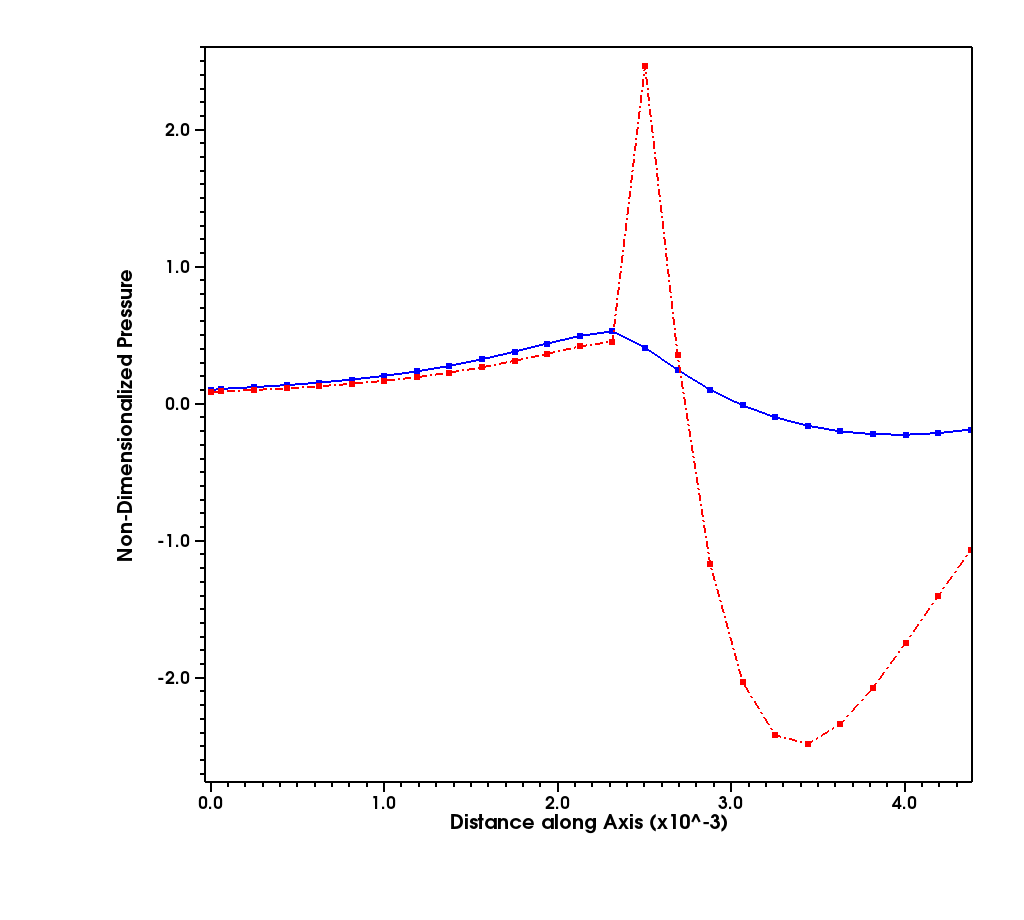
\includegraphics[width=0.45\textwidth]{Figures/Sagar/16ppd_MC_vc_NON-MC.png} &
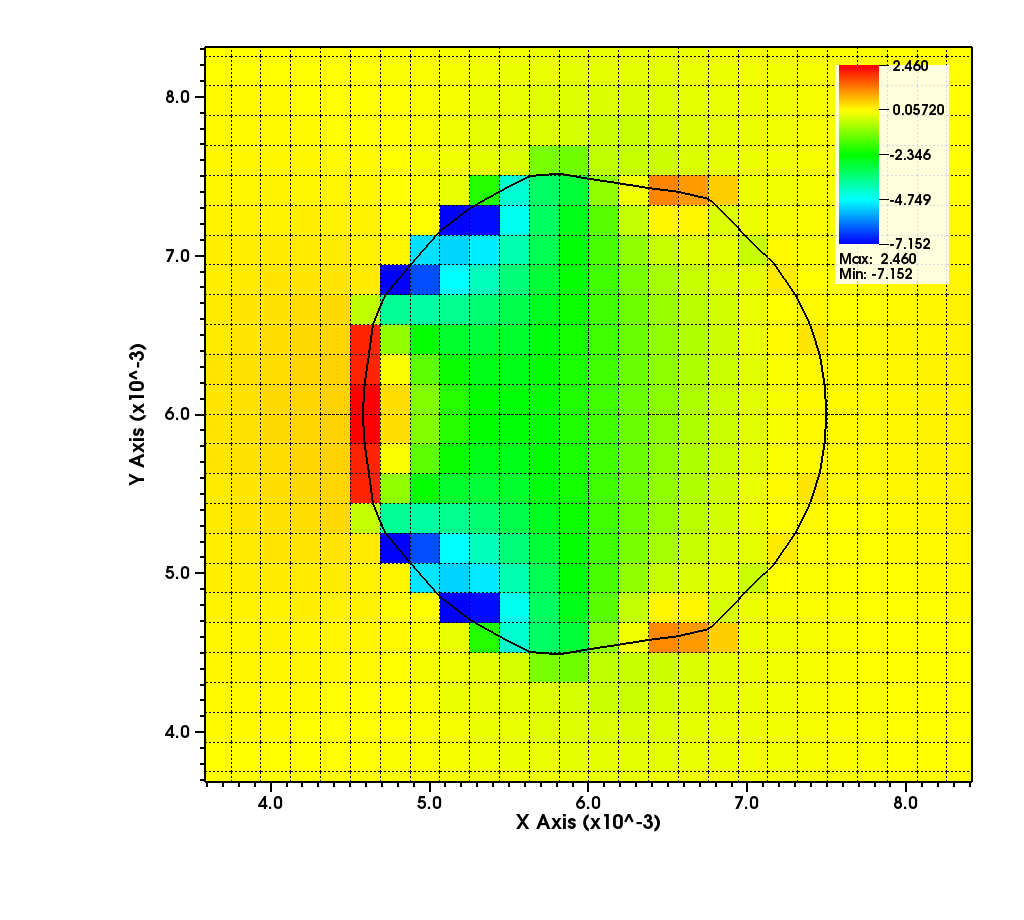
\includegraphics[width=0.45\textwidth]
{Figures/Sagar/non_MC_16ppd_pressure_corrected.png}\\
(a) & (b)
\end{tabular}
\end{center}
\caption{The origin of the pressure peak in the front of the droplet. 
(a) The profile of the pressure on the axis a few timesteps after initialisation 
with the standard, non-momentum conserving method (red) and the present method 
(blue). (b) The pressure distribution immediately after the start of the simulation 
using the standard, non-momentum-conserving method. The pressure peak does
not result yet in the formation of a dimple. In all figures  $D/h = 16$.}
\label{FengXiao}
\end{figure}
% -----

% -----
\begin{figure}
\begin{center}
\begin{tabular}{cc}
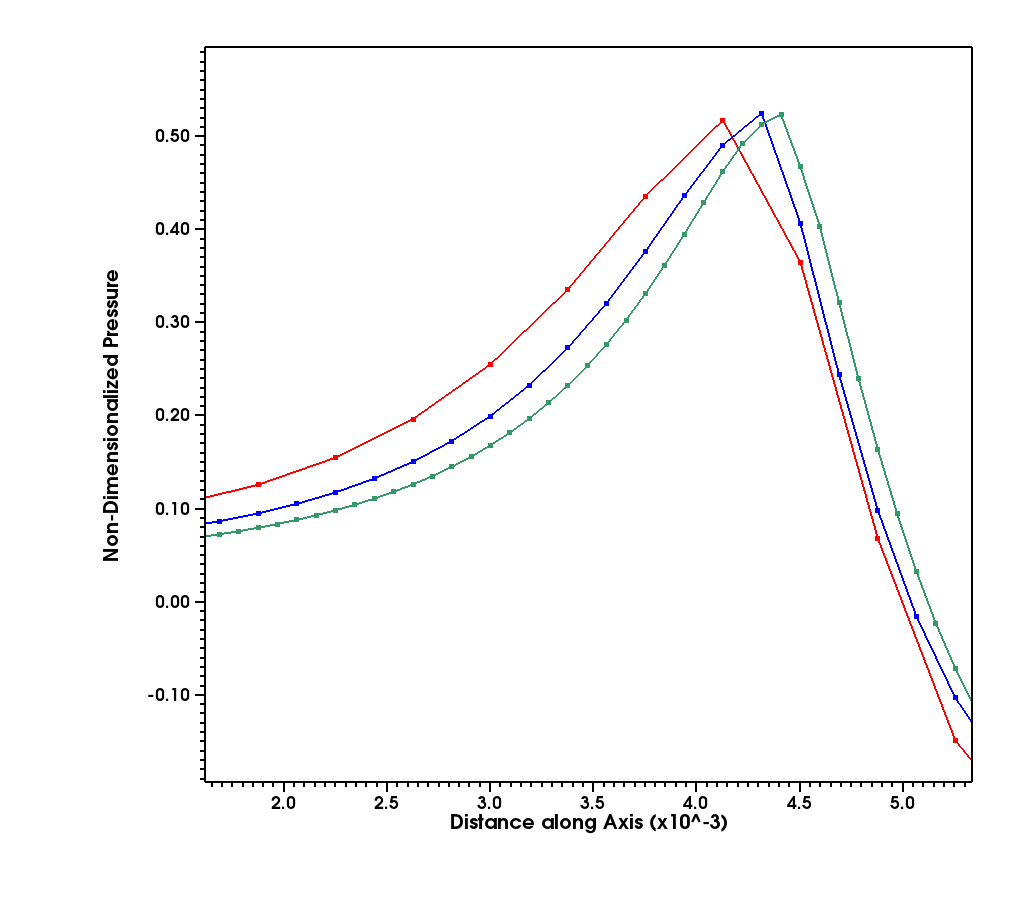
\includegraphics[width=0.45\textwidth]{Figures/Sagar/pressure_rd_MC.png} &
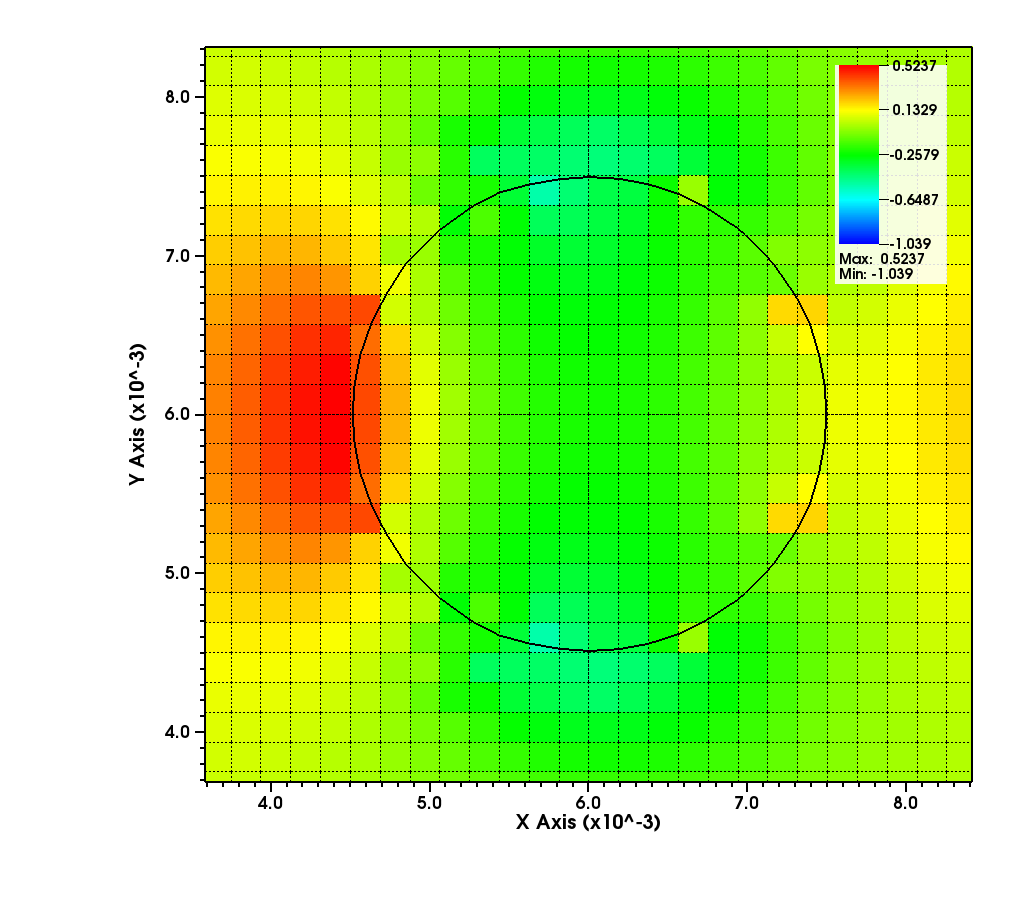
\includegraphics[width=0.45\textwidth]
{Figures/Sagar/16ppd_pressure_corrected.png}\\
(a) & (b)
\end{tabular}
\end{center}
\caption{ (a) The pressure profile on the axis a few timesteps after 
initialisation with the present 
method at various resolutions: $D/h = 8$ (red) , $16$ (blue) and $32$ (green). 
(b) The pressure distribution immediately after the start of the simulation 
using the present method and   $D/h = 16$.}
\label{FengXiao_corrected}
\end{figure}
% -----

\vspace*{0.2cm}

\begin{figure}[!h]
\begin{center}
\begin{tabular}{cc}
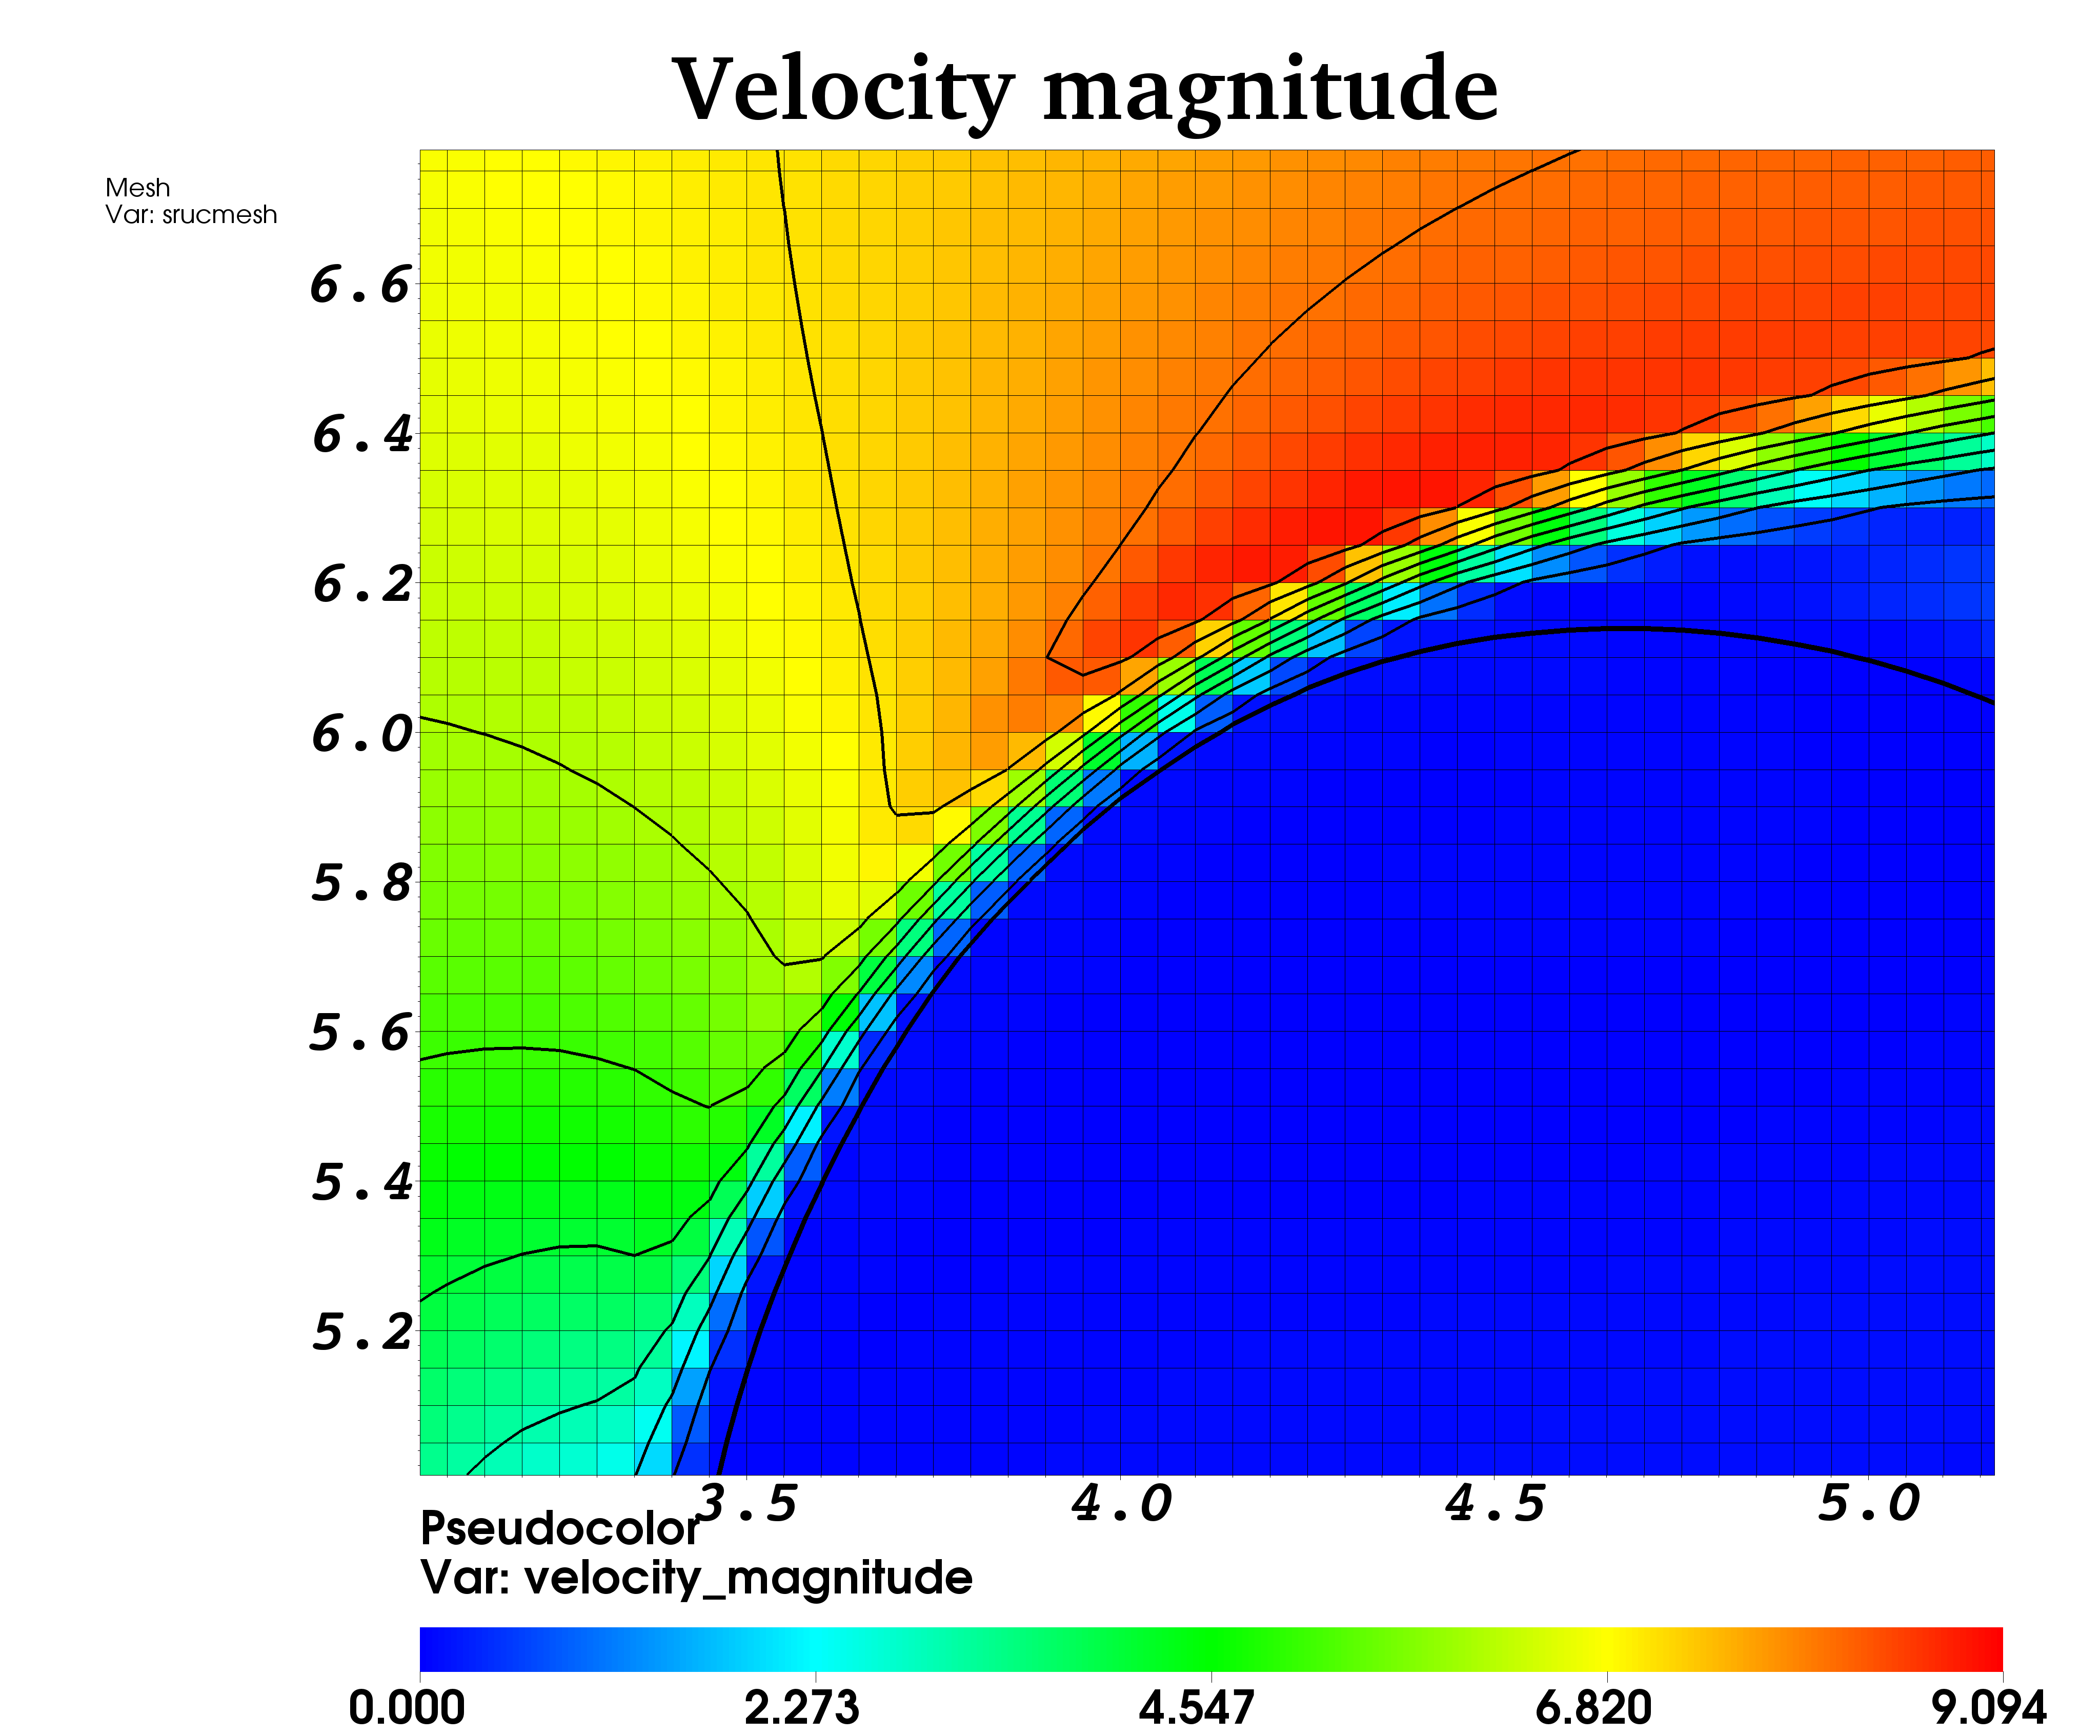
\includegraphics[width=0.42\textwidth]{Figures/vel.png}
& 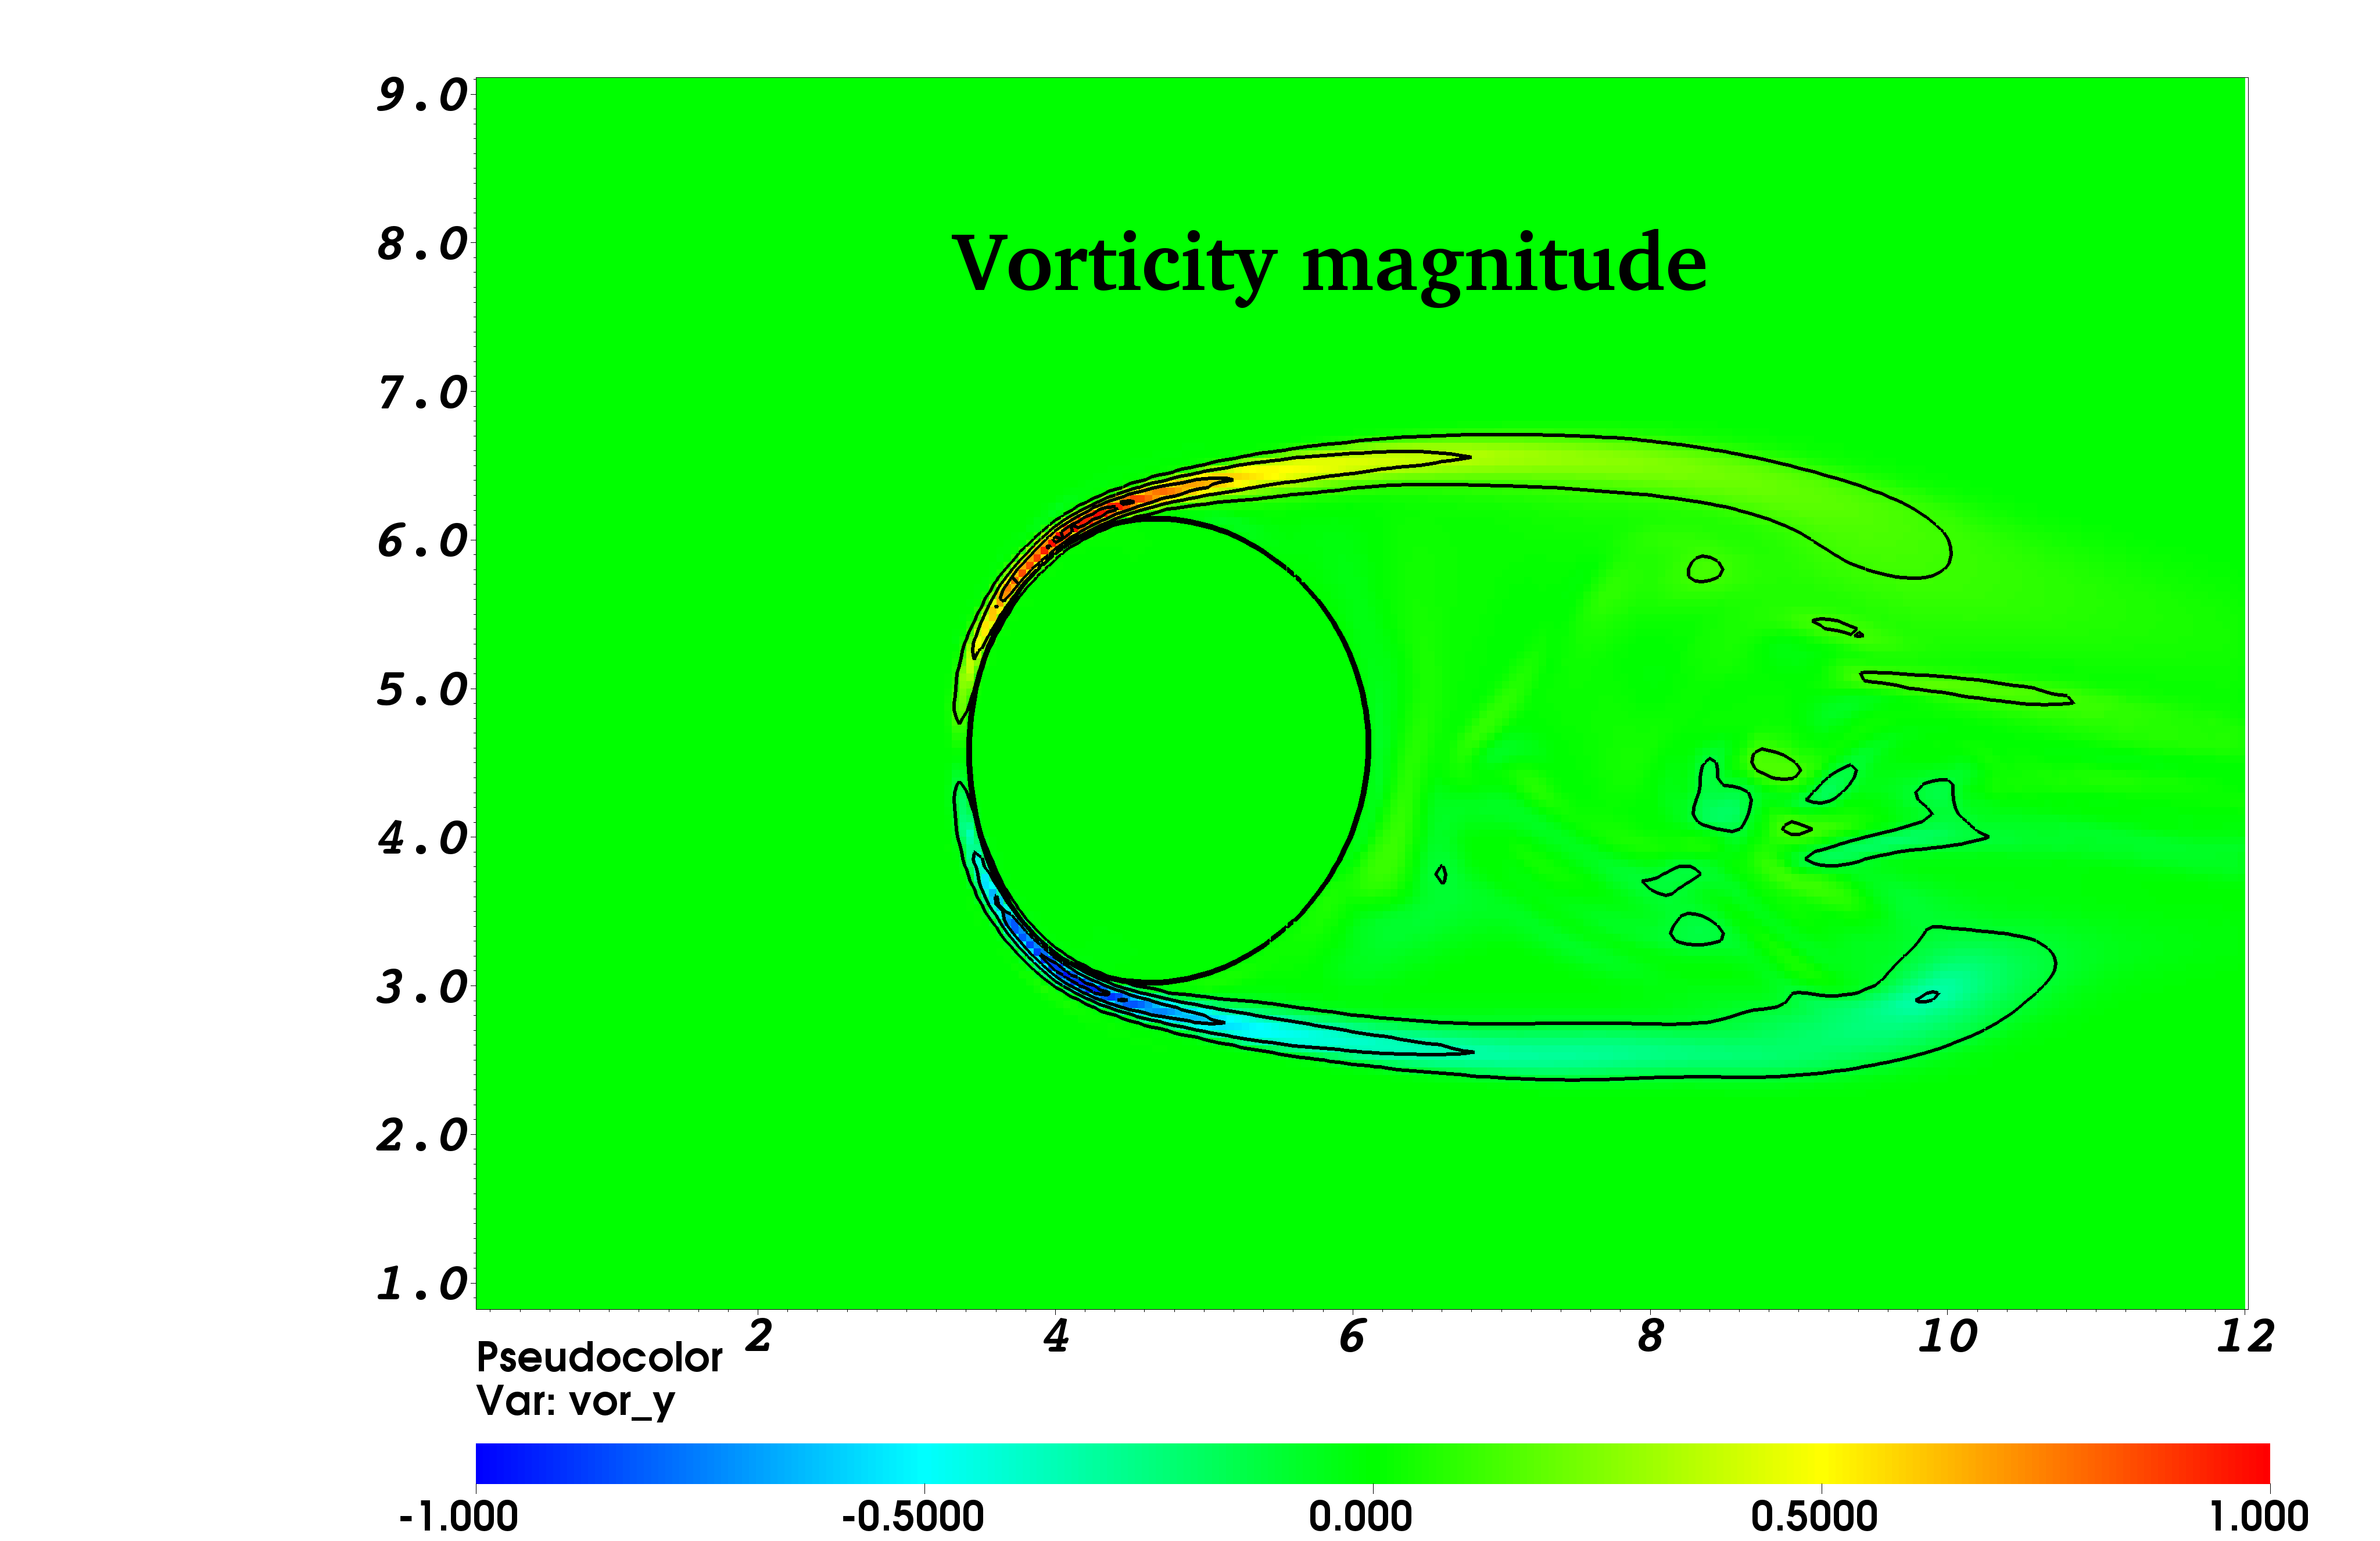
\includegraphics[width=0.48\textwidth]{Figures/vort.png} \\
(a) & (b)
\end{tabular}
\end{center}
\caption{Flow field around the 3 mm droplet with 60 grid points per diameter. 
(a) The velocity magnitude. It is seen that even at this highest resolution 
there are only three points in the boundary layer. (b) The vorticity magnitude. 
The marked separation of the boundary layers is observed with 
a more complex vortical region in the wake.}
\label{magn}
\end{figure}
% -----
\newcommand\DDD{{\cal D}}

Visualisation of the flow around the droplets (Figure \ref{magn}) elucidates the challenging nature of the flow configuration, even with such an apparently simple physical problem. As one can observe, the boundary layers are extremely thin, hence questioning our approximation that fluid velocity is continuous across the interface. We observe that applying the numerical method described in this paper brings a considerable and systematic improvement over a range of different flux limiters (WENO,ENO, Superbee, QUICK, Verstappen) and CFL numbers, as evidenced by comparing the figures \ref{FengXiao} and \ref{FengXiao_corrected}. To summarize, the simulations broadly fall in three categories: 

\begin{enumerate}
	\item They blow up anyway even while applying the present method
	\item They keep physical values of the kinetic energy and render smooth interfacial shapes.
	\item They have a marked peak in kinetic energy as a function of time, associated with massively deformed interface shapes, 
\end{enumerate}

Regarding the first two points made above, we find that certain combinations of the advection scheme (CIAM/WY) and the flux limiter (ENO/WENO/Superbee/Verstappen/QUICK) display more numerical stability that the others, in particular, the most stable combinations of schemes are CIAM advection with Superbee limiter and the WY advection with QUICK limiter. As a minor remark, the CIAM advection with the Superbee limiter also appears to be quite diffusive. The third point highlights the systematic behavior of the simulations that are carried out without applying the present momentum-conserving method. 

\vspace*{0.2cm}

Subsequently, we evaluate the performance of the present method as a function of droplet resolution. We carry out simulations corresponding to $D/h = 8, 16, 32 \text{and} 64 $, while keeping the same value for the inflow velocity. The quantities of interest while evaluating the method are conservation of mass and momentum in the domain, temporal evolution of the droplet kinetic energy and the moment of inertia of the droplet. For the latter, we use as a descriptor of the shape the three moments of inertia $I_m$ defined by
\be
I_m = \int_\DDD H x_m^2 {\rm d}\X \;, \quad  1 \le m \le 3,
\nd

where $\DDD$ is the domain used for the computation and $x_m$ is relative to the center of mass. 


In order to validate our simulation, we study the convergence upon grid 
refinement. Three grids are used, with $D/h=15,\,30$ and $60$. A $12$-mm 
cubic box is used with the $3$-mm droplet at the center.  
We study the convergence of the terminal velocity and that of the shape. 
For the latter, we use as a descriptor of the shape the three moments of 
inertia $I_m$ defined by
\be
I_m = \int_\DDD H x_m^2 {\rm d}\X \;, \quad  1 \le m \le 3,
\nd
where $\DDD$ is the domain used for the computation and $x_m$ is relative to
the center of mass. The convergence of the moments of inertia and terminal 
velocity is shown on Figure \ref{converge}. The velocity seems to converge 
to a value around $7\, m/s$, to be compared with a value of $8.06 \,m/s$ 
found by the authors of ref. \cite{gunn1949terminal}. 
This is not surprising since the experimental terminal velocity would be 
modified for a droplet constrained in a finite-size box.
% -----
\begin{figure}
\begin{center}
\begin{tabular}{cc}
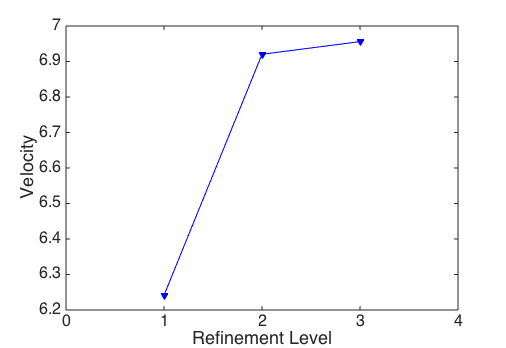
\includegraphics[width=0.45\textwidth]{Figures/veloconv.png}
& 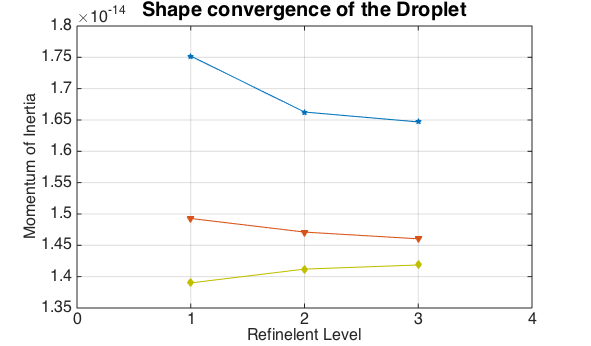
\includegraphics[width=0.45\textwidth]{Figures/shapeconv.png} \\
(a) & (b)
\end{tabular}
\end{center}
\caption{Convergence of simulations. (a) Evolution of the terminal velocity 
with grid refinement. (b) Evolution of the three moments of inertia with 
grid refinement.}
\label{converge}
\end{figure}
% -----
% -----
\begin{figure}
\begin{center}
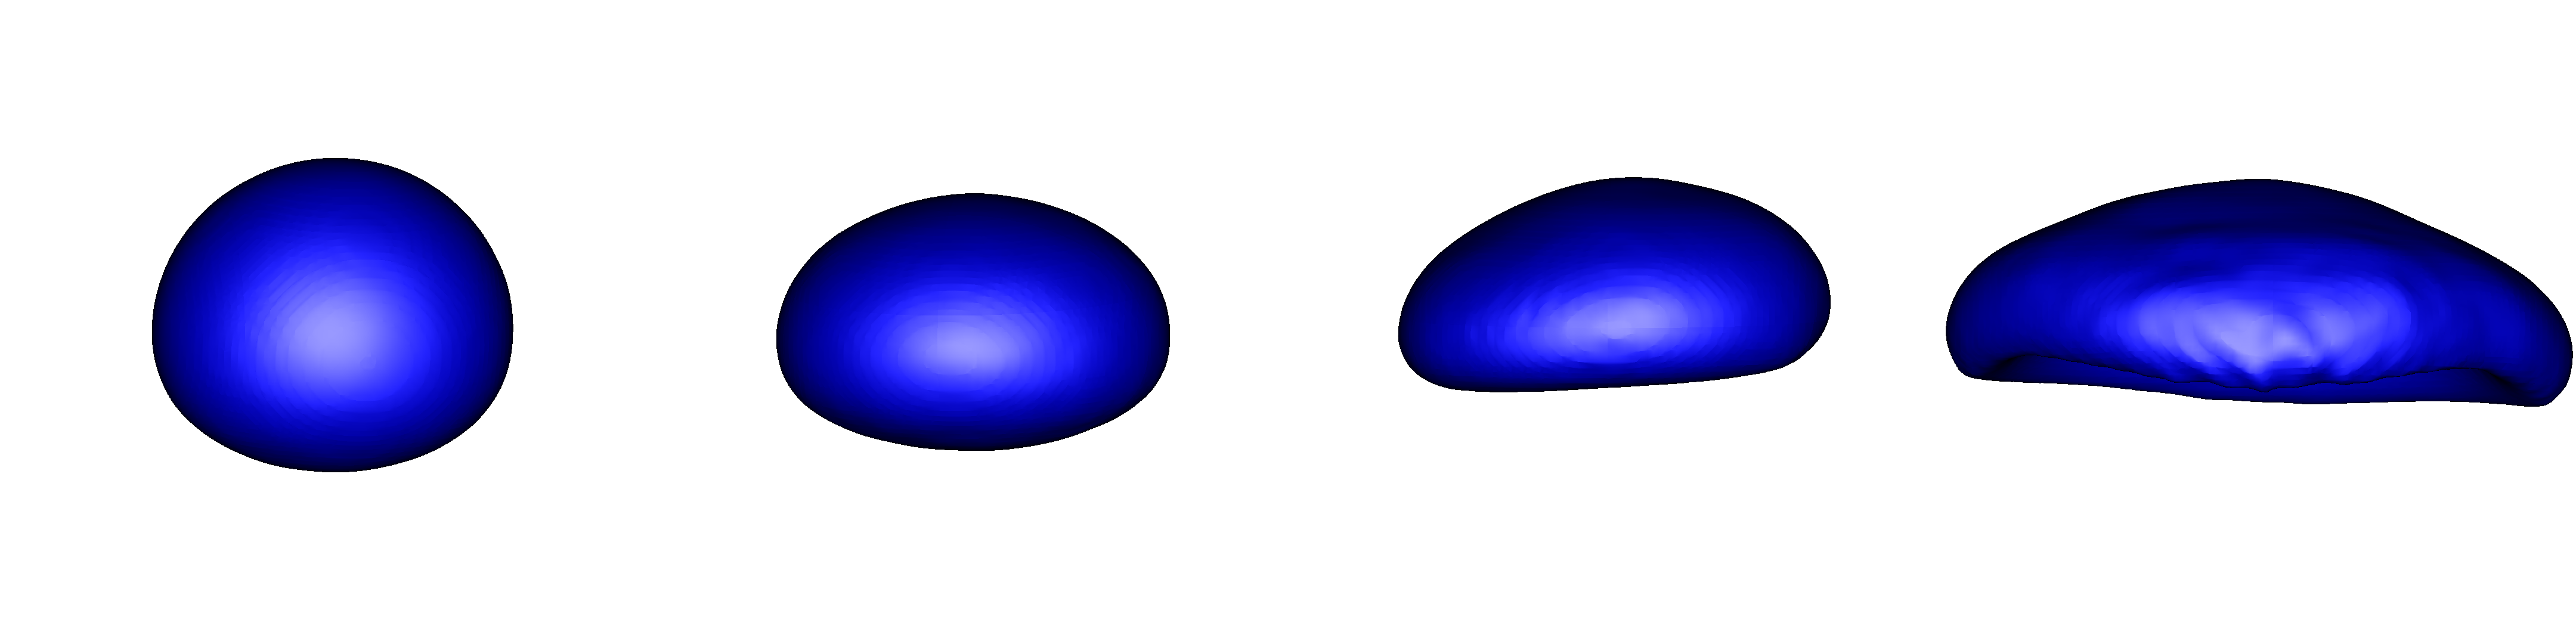
\includegraphics[width=0.99\textwidth]{Figures/flatten.png}
%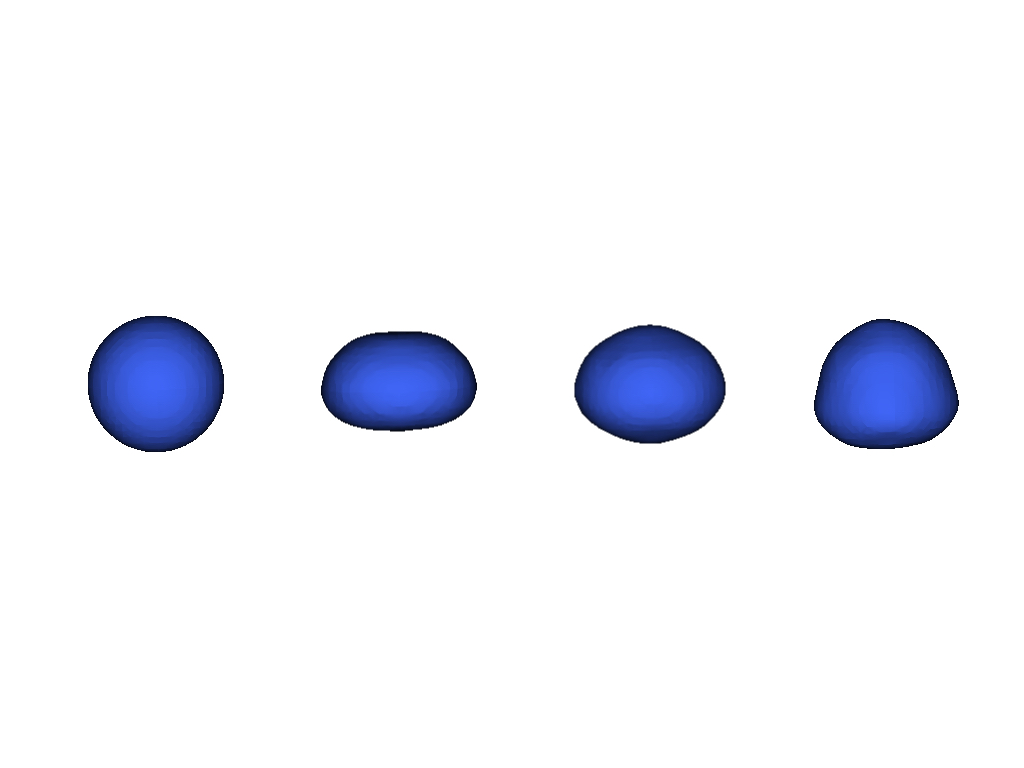
\includegraphics[width=0.99\textwidth]{Figures/Sagar/fig14-001.jpeg}
\end{center}
\caption{Flattening of the droplet with increasing equivalent diameter 
(see text). From left to right $D_e=3, \,4.6,\, 6.4$ and $8\, mm$.}
\label{flatten}
\end{figure}
% -----
From the values of the moments of inertia, the horizontal and vertical 
extents of the droplet (respectively $D_r$ and $D_x$) can be found 
and compared to the values found by the authors of \cite{Reyssat:2007ko}. 
We find $D_r=3.1 \,mm$ and $D_x=2.6 \,mm$, while ref. \cite{Reyssat:2007ko} 
concludes that drops are quasi-spherical for an equivalent diameter 
$D_e \le l_c$ and deformed for $D_e > l_c$, where $l_c =(\sigma/\rho g)^{1/2}$ 
is the capillary length, $l_c = 2.7 \,mm$ for water. 
Indeed repeating the simulations for larger drops we find increased 
flattening as shown on Figure \ref{flatten}. 
%
%\clearpage

% Slightly less stable methods result when one takes $\hat x = x_i$. 
% In that case we observe at low resolution ($D/h=15$) the energy spike shown 
% in Figure \ref{lowres}. The energy spike is 
% associated with a moving bump on the droplet. Using a higher resolution 
% of $D/h=30$ makes the energy spike disappear. 
% Switching to the shifting of the interpolation point $\hat x$ described in 
% Section \ref{tunedinter}, even more stable behavior is observed, down 
% to resolutions of $D/h=8$. 
% -----
% \begin{figure}
% \begin{center}
% \begin{tabular}{cc}
% 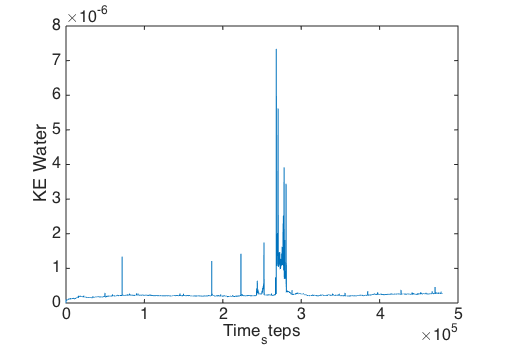
\includegraphics[width=0.5\textwidth]{Figures/KE.png}
% & 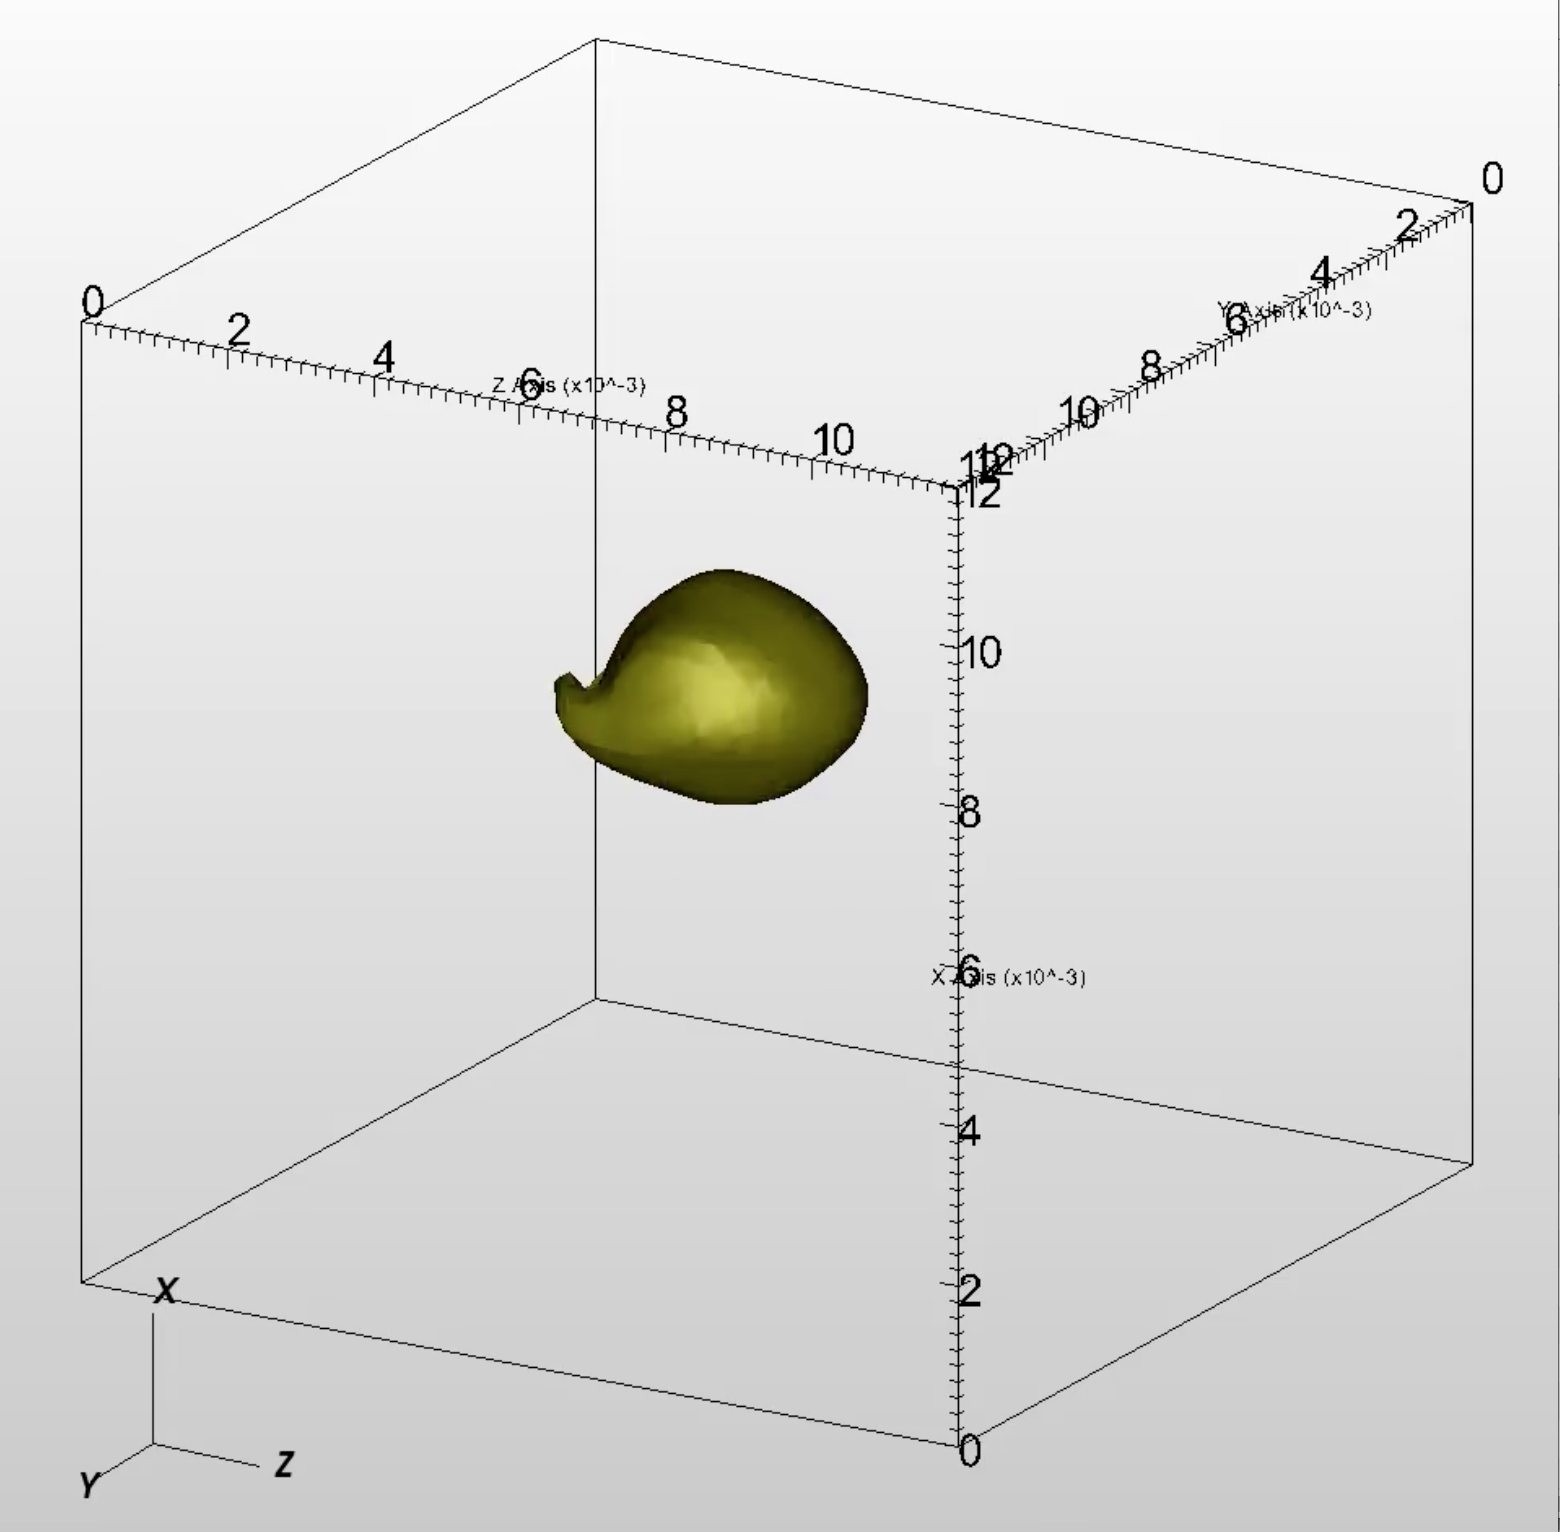
\includegraphics[width=0.4\textwidth]{Figures/bump.png} \\
% (a) & (b)
% \end{tabular}
% \end{center}
% \caption{Effect of a slightly unstable setup. (a) The kinetic energy 
% as a function of time exhibits several
% spikes (b) A snapshot of the simulation at the instant of the formation 
% of the first spike. A pointed
% bump forms on the droplet and starts rotating rapidly.}
% \label{lowres}
% \end{figure}
% -----

